% !TeX spellcheck = it_IT
\section{Mobile Network}

\subsection{Introduzione alle reti mobili}

\paragraph{Pre-Cellulare:} Prima degli anni '80 esistenza un servizio di telefonia mobile con trasmettitori e ricevitori ad elevata potenza, con 25 canali e 80km di raggio di copertura. Capacità insufficiente per fornire un servizio di telefonia (voce) comparabile con i servizi di telefonia fissi.\\

L'idea dietro la rete cellulare invece è usare \textbf{molteplici trasmettitori} con una potenza "bassa", minore di 100W. Meno potenza, meno raggio di copertura: l'area viene divisa in celle (da qui "cellulare"), ognuna con una propria antenna (o più).\\

Ogni cella è servita da una \textbf{Base Station (BS)}:
\begin{itemize}
	\item Trasmettitore
	\item Ricevitore
	\item Unità di controllo
\end{itemize}
Può operare in licensed/unlicensed spectrum.\\

La progressione è:
\begin{itemize}
	\item 1980 \textbf{1G Advanced Mobile Phone Service (AMPS)}: Voce analogica in mobilità
	\item 1990 \textbf{2G Global System for Mobile Communication (GSM)}: Voce digitale (compressa, \dots), prima rete globale
	\item 2000 \textbf{3G Universal Mobile Telecommunications System (UMTS)}: Introduce i servizi internet
	\item 2010 \textbf{4G Long Term Evolution (LTE)}: convergenza IP e aumento delle prestazioni
	\item 2020 \textbf{5G}: Networks softwarization \& virtualization, slicing \& bassa latenza
	\item 2030 \textbf{6G}: Network intelligence (AI all'interno della rete, ottimizzazione secondo AI)
\end{itemize}

Gli standard della rete cellulare si possono vedere su \href{https://www.3gpp.org/specifications-technologies/releases}{\texttt{Third Generation Partnership Project (3GPP)}}. Sono tutte le release su cui si basano i rilasci commerciali.\\

\paragraph{Base Station BS:} Un esempio di BS può essere
\begin{center}
	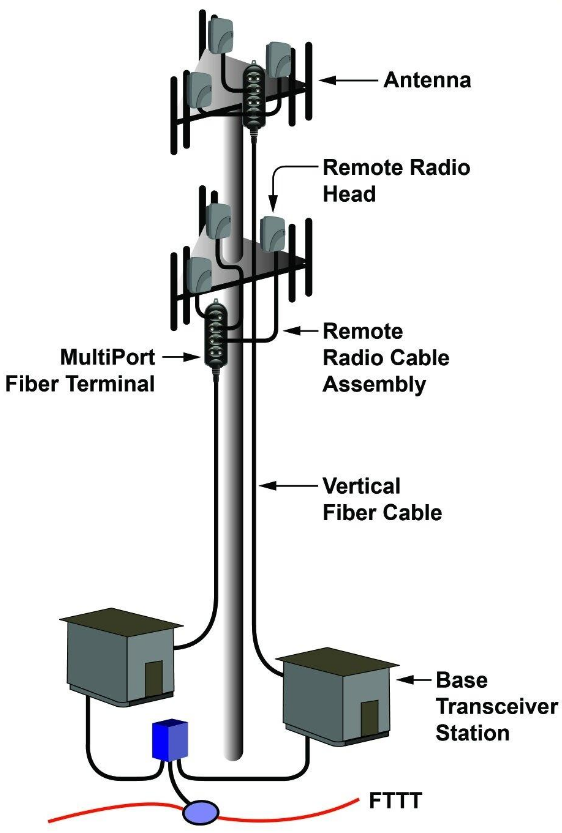
\includegraphics[width=0.4\linewidth]{img/mobile/1BS}
\end{center}

Le componenti sono:
\begin{itemize}
	\item \textbf{Antenna}: trasmette e riceve onde radio
	\item \textbf{Remote radio head}: riceve i segnali analogici e li converte in digitale e viceversa; vicino all'antenna per ridurre la perdita di segnale nei cavi
	\item \textbf{Remote radio cable assembly}: gruppo di cavi che fornisce alimentazione e/o collegamento dati tra la stazione base e i Remote Radio Heads
	\item \textbf{MultiPort Fiber Terminal}: punto di terminazione o distribuzione in cui la fibra ottica in entrata viene divisa o collegata a più uscite per servire le diverse RRH. In pratica, funge da "scatola di giunzione" per organizzare e connettere i vari cavi in fibra destinati ai moduli radio remoti
	\item \textbf{Base Transceiver Station (BTS)}:L'elemento principale dell'infrastruttura della rete mobile, gestisce il traffico dati e vocale, coordina i protocolli radio, si interfaccia con la rete di trasporto verso il core network dell'operatore e invia i segnali digitali agli RRH. Al suo interno si trova l'elettronica di baseband (elaborazione del segnale, modulazione/demodulazione, protocolli) e vari componenti di controllo
\end{itemize}

\subsubsection{Organizzazione Geometrica delle Celle}

Bisogna capire come disporre le celle. I requisiti sono:
\begin{itemize}
	\item coprire "bene" l'area
	\item avere una disposizione uniforme
\end{itemize}

Una buona disposizione usa celle esagonali per una copertura e disposizione uniforme. Ovviamente si tratta della disposizione ideale, nella realtà ci sono dei vincoli, di posizionamento e diffusione del segnale.\\

\paragraph{Riuso delle frequenze:} Si ha il problema di avere celle vicine con la stessa banda di frequenza: dispositivi sui bordi ricevono dati da entrambe le celle. \\

La prima soluzione è usare \textbf{frequenze diverse tra celle vicine}, ma servono più bande (licensed spectrum, costa e ne uso solo una parte per volta). 2G opera in questo modo.\\

Un'altra soluzione, per non "sprecare" banda, è usare la stessa frequenza e \textbf{tecniche di codifica} per evitare le interferenze tra celle vicine (\textbf{CDMA}).\\

L'ultima soluzione è:
\begin{itemize}
	\item al \textbf{centro} di ogni cella usare l'\textbf{intera ban}da disponibile (tranne un pezzo), per gli utenti interni
	\item al \textbf{bordo}, \textbf{celle vicine} hanno \textbf{frequenze diverse}
\end{itemize}

Questo permette bandwidth maggiore per utenti interni ma richiede un sofisticato controllo di potenza e coordinamento tra BS (4G e 5G). Bisogna posizionare all'interno della cella i dispositivi in maniera abbastanza precisa per stabilire che frequenze utilizzare. \\

%fino s16
%End L15